\begin{table}[h]
\centering
\label{data_sources}
\caption{Origins of labeled training data}
\begin{tabular}{|r|r|l|}
\hline
Amount & Label & Origin \\ \hline
9 & DATA & Manual Google search for Open Data
repositories \\ \hline
82 & DATA & Repositories of GitHub user `datasets' \\ \hline
17 & EDU & GitHub Search for ``course, material'' \\ \hline
17 & DOCS & GitHub Search for ``documentation'' \\ \hline
423 & WEB & Google Search for ``site:.github.io'' \\ \hline
58 & HW & GitHub Search for ``homework, assignments,
solution'' \\ \hline
13 & DEV & Showcases ``Virtual Reality'' \\ \hline
12 & DEV & Showcases ``Software Development Tools'' \\ \hline
14 & DEV & Showcases ``Front-end JavaScript frameworks'' \\ \hline
20 & DEV & Showcases ``DevOps tools'' \\ \hline
16 & DEV & Showcases ``Text editors'' \\ \hline
24 & DEV & Showcases ``Game Engines'' \\ \hline
27 & DEV & Showcases ``Web Application Frameworks'' \\ \hline
42 & DEV & Showcases ``Programming Languages'' \\ \hline
180 & DOCS & GitHub Repo Content: awesome-awesomeness \\ \hline
6 & DATA & Showcases ``Open Data'' \\ \hline
86 & HW & Github Search for ``homework, solution'' \\ \hline
\end{tabular}
\end{table}

\begin{figure}[h]
	\centering
		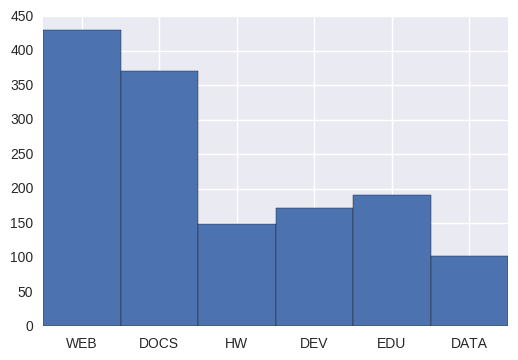
\includegraphics[width=10cm]{graphics/training_data_distribution.png}
	\caption{Training Data Distribution}
	\label{training_data_distribution}
\end{figure}


\begin{figure}[h]
	\centering
		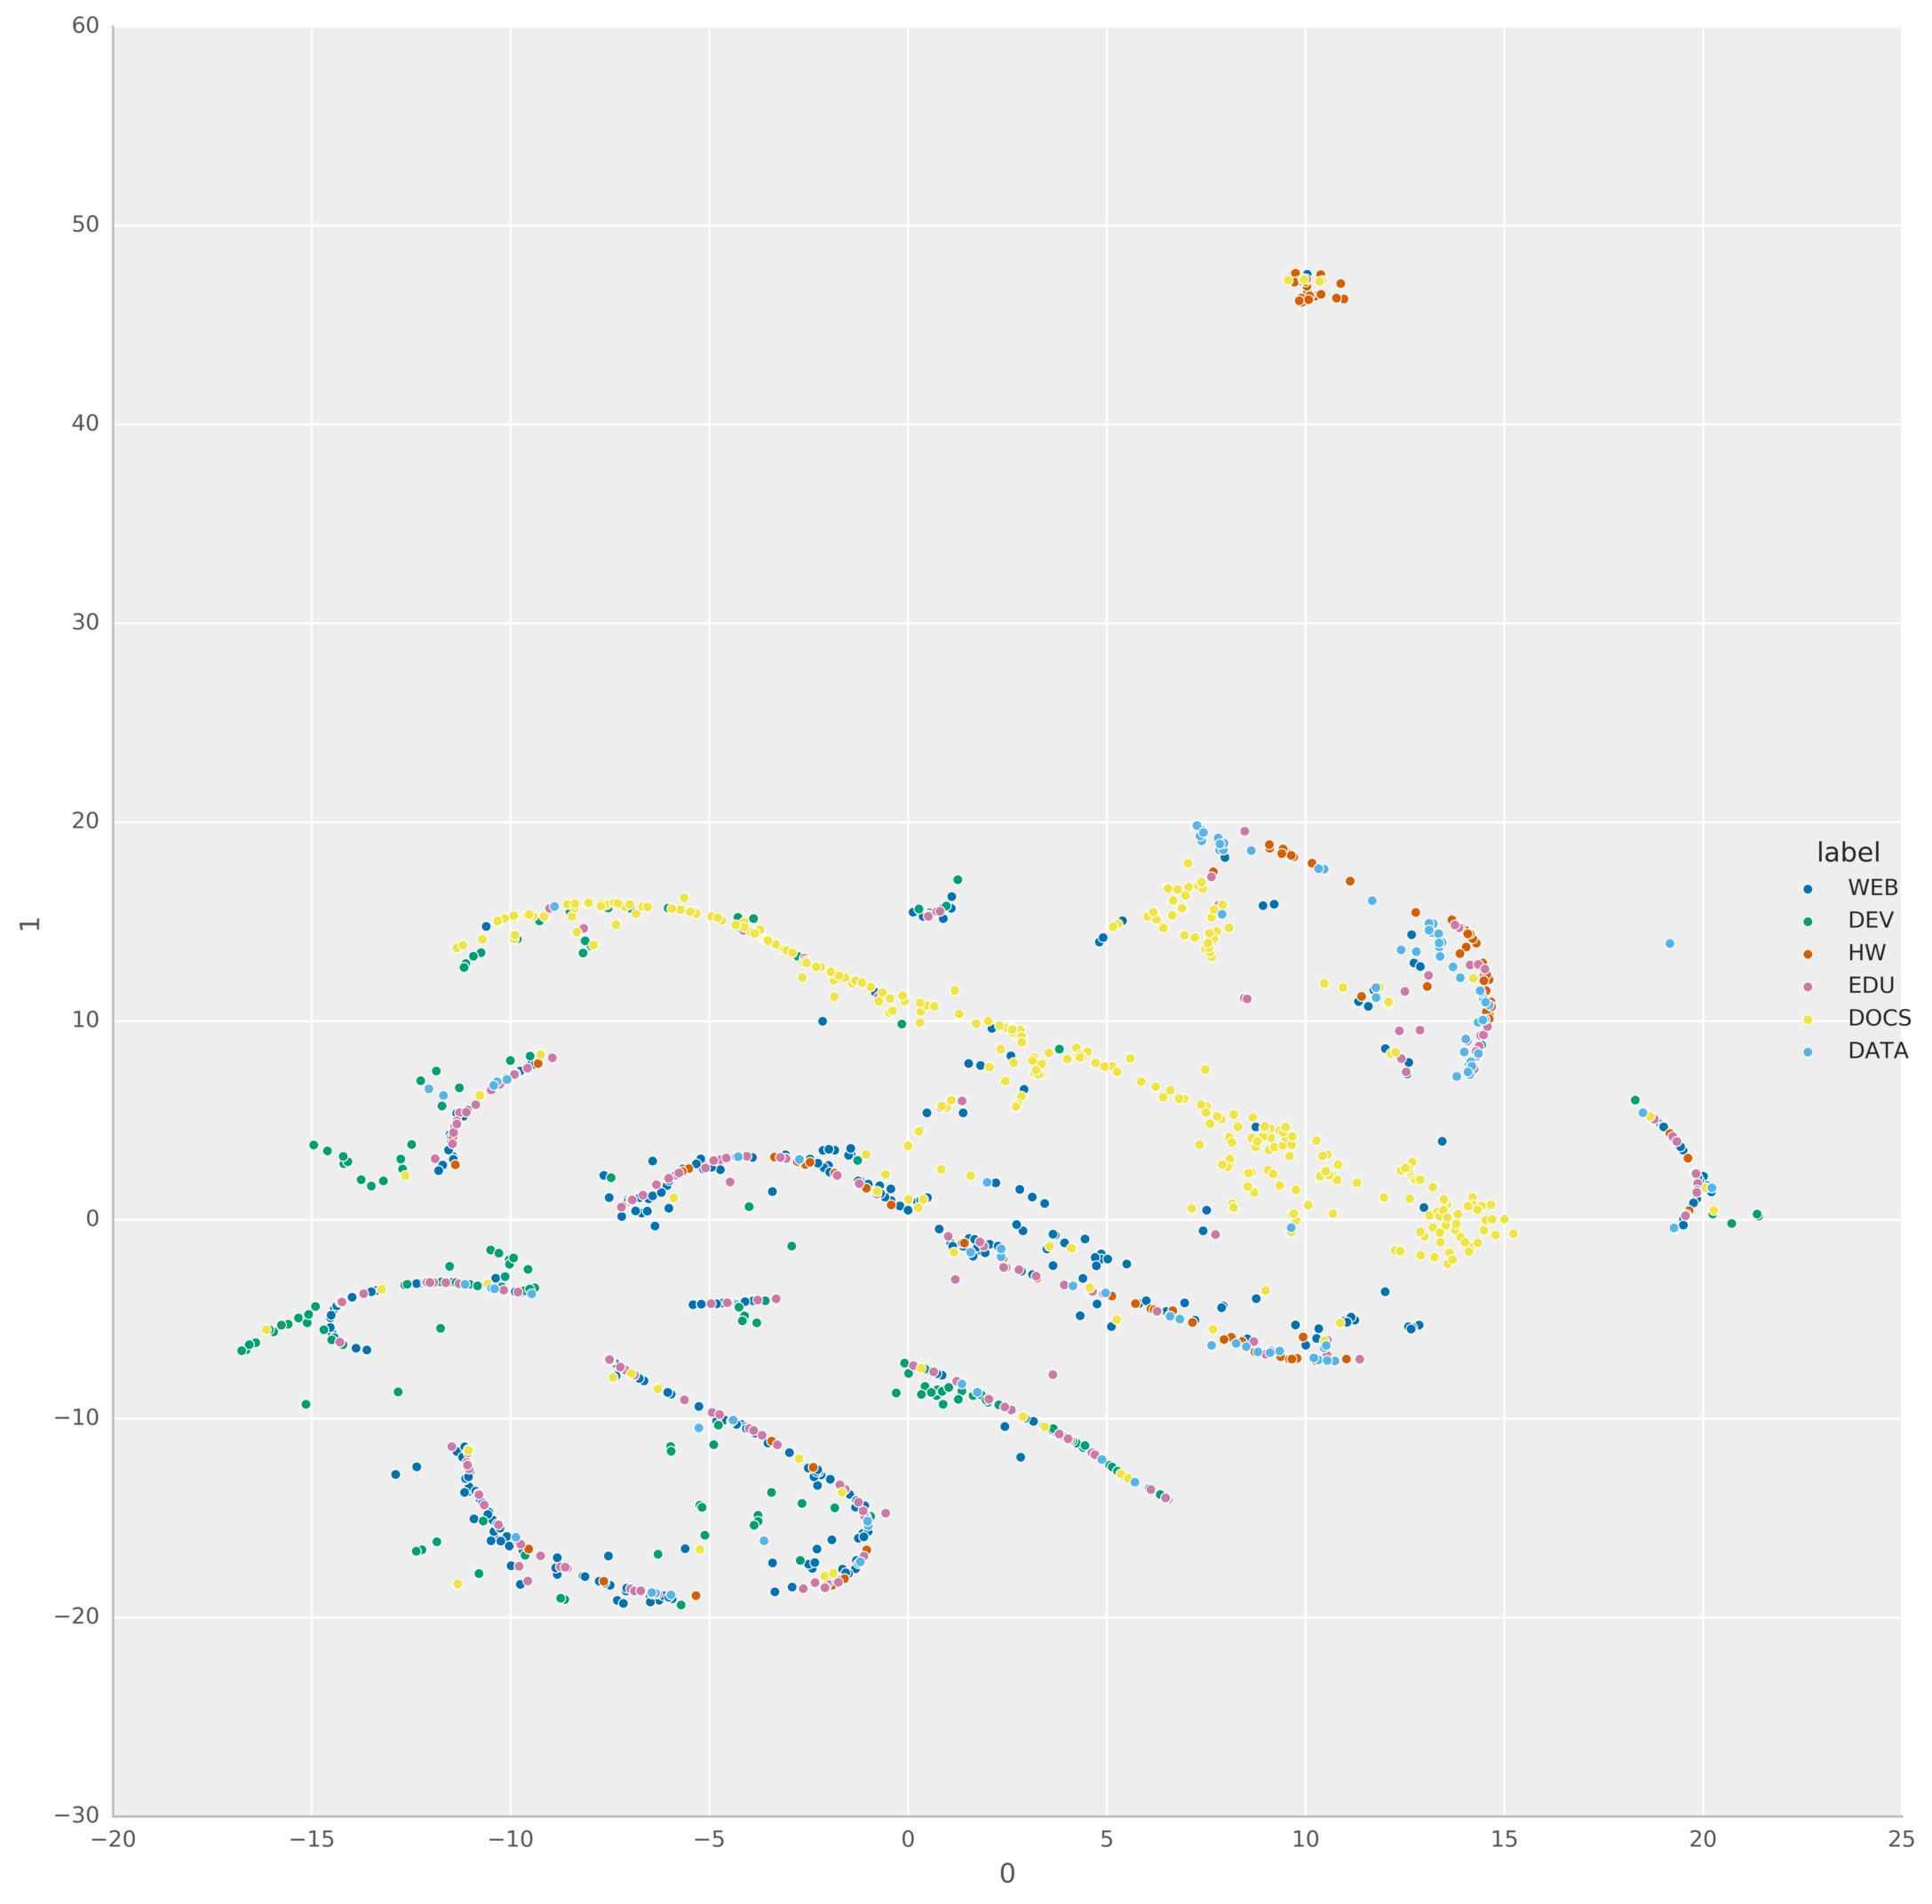
\includegraphics[width=18cm]{graphics/t-sne-training-data.png}
	\caption{Distribution of the labeled data entries using t-SNE}
	\label{t-sne-training-data}
\end{figure}


\begin{figure}[h]
	\centering
		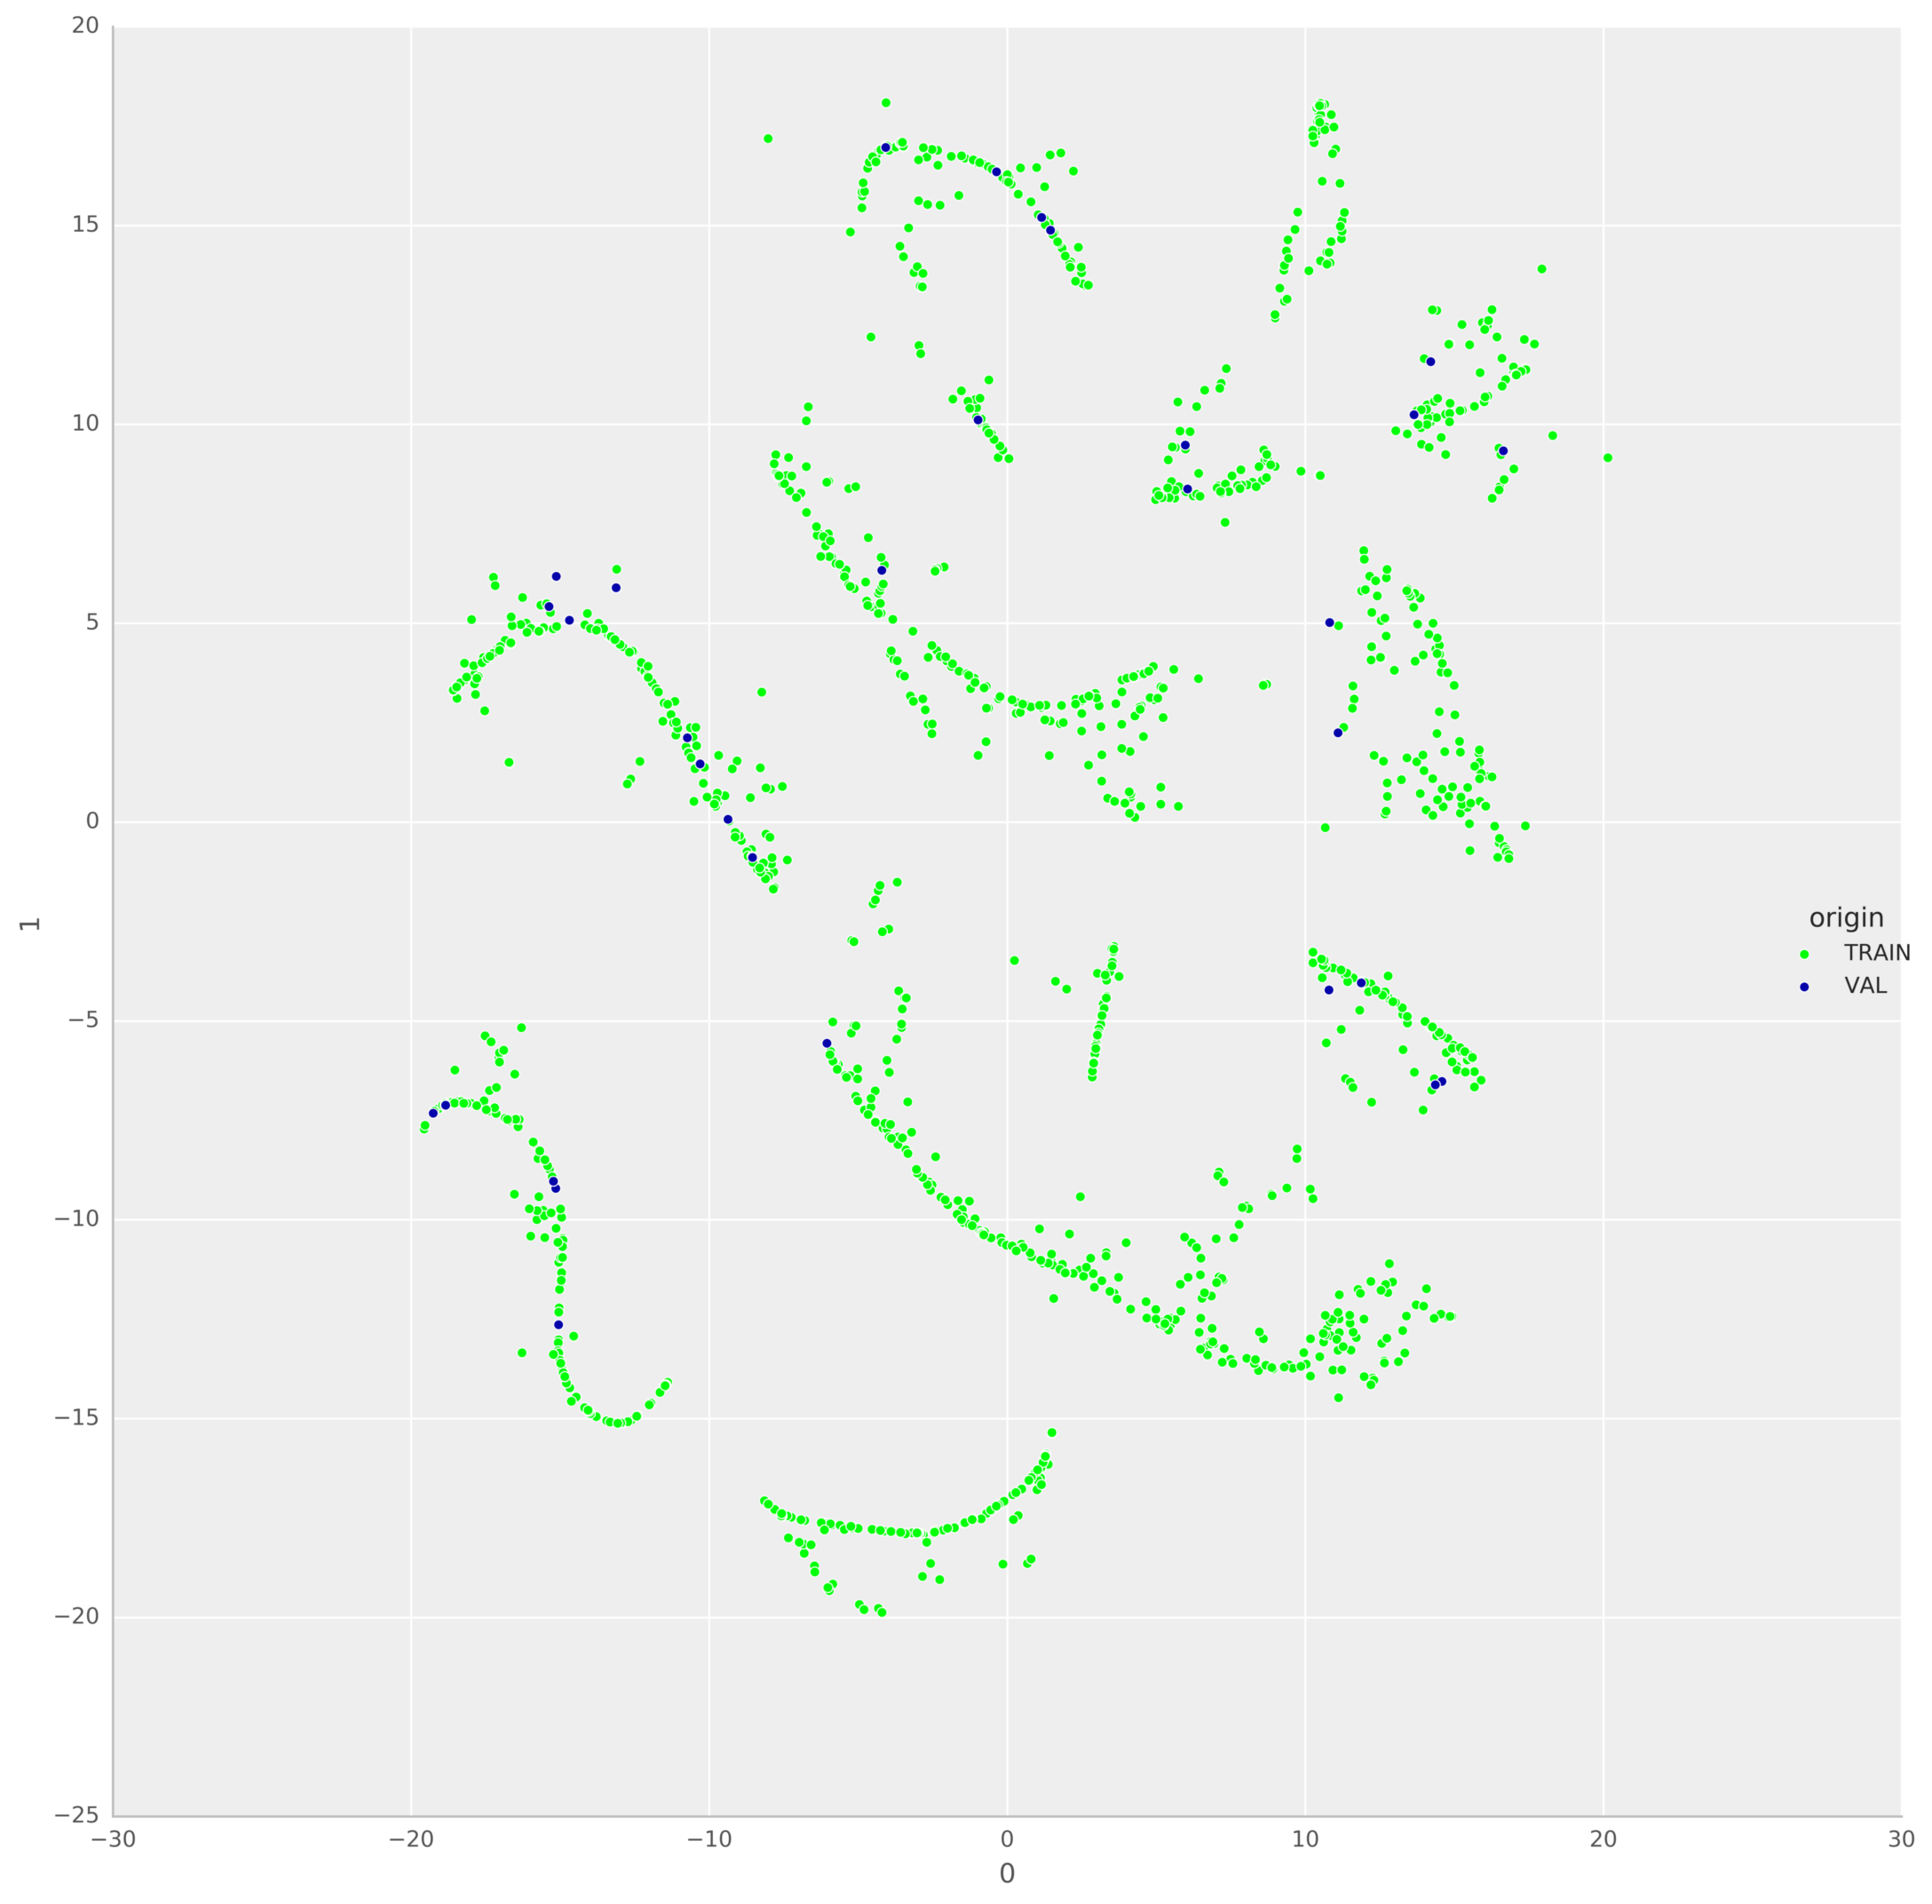
\includegraphics[width=18cm]{graphics/t-sne-validation-data.png}
	\caption{Distribution of the validation data entries using t-SNE}
	\label{t-sne-validation-data}
\end{figure}


\begin{figure}[h]
	\centering
		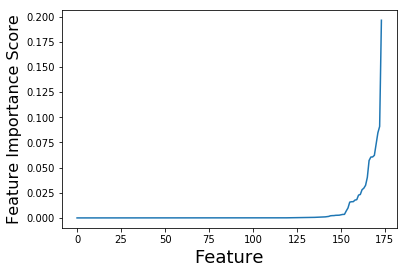
\includegraphics[width=12cm]{graphics/feature_importance_numeric.png}
	\caption{Feature Importance Scores for Numeric Features}
	\label{feature_importance_numeric_graphic}
\end{figure}

\begin{table}[h]
	\centering
	\caption{Top 20 Most Important Numeric Features}
	\label{feature_importance_numeric}
	\begin{tabular}{|l|l|l|l|}
	\hline
		Feature Names & Scores & Feature Names & Scores \\ \hline
		isOwnerHomepage  &   0.1793 & hasHomepage & 0.1297 \\ \hline
		stargazers  &   0.0726 & mentionableUsers & 0.0642 \\ \hline
		size  &   0.0581 & watchers & 0.0561 \\ \hline
		commitsCount  &   0.0492 & closed\_issues & 0.0415 \\ \hline
		merged\_pull\_requests  &   0.0389 & open\_issues & 0.0379 \\ \hline
		forks  &   0.0376 & closed\_pull\_requests & 0.0368 \\ \hline
		tagsCount  &   0.0245 & branchesCount & 0.0239 \\ \hline
		hasTravisConfig  &   0.0235 & open\_pull\_requests & 0.0223 \\ \hline
		releasesCount  &   0.0214 & hasLicense & 0.0148 \\ \hline
		hasCiConfig  &   0.0124 & LANGUAGE\_Python & 0.0090 \\ \hline
	\end{tabular}
\end{table}
